% From course hosting to adaptive learning: ALP — a reference platform and plugin architecture for learner memory and multimodal delivery
% arXiv-ready draft
\documentclass[10pt,twocolumn]{article}
\usepackage[utf8]{inputenc}
\usepackage[T1]{fontenc}
\usepackage{url}
\usepackage{hyperref}
\usepackage{graphicx}
\usepackage{booktabs}
\usepackage{amsmath}
\usepackage[margin=1in]{geometry}
\usepackage{tikz}
\usetikzlibrary{positioning,shapes.geometric,arrows.meta,fit,backgrounds}
\hypersetup{colorlinks=true,linkcolor=blue,citecolor=blue,urlcolor=blue}

\title{From Course Hosting to Adaptive Learning: An AI-Native Platform and Plugin Architecture for Learner Memory and Multimodal Delivery}
\author{
  Dhanikesh Karunanithi\\
  \texttt{Sudar / ALP Project}\\
  \url{https://github.com/lorddannykay/ByteOS}
}
\date{2026}

\begin{document}
\maketitle

\begin{abstract}
Traditional learning management systems (LMSs) deliver static content with no longitudinal learner model or adaptive tutoring, while intelligent tutoring systems (ITS) that do adapt remain research prototypes or narrow-domain tools. We present an AI-native learning system with two contributions: (1) a full reference platform that combines authoring, delivery, and intelligence with a persistent Digital Learner Twin, adaptive sequencing, multimodal delivery (text, video, audio, mindmap, flashcards, and more), and an AI tutor with longitudinal memory; and (2) an architecture---which we call the Adaptive Learning Layer (ALP)---by which these components can be deployed as standalone plugins to turn existing LMSs into adaptive, memory-aware learning experience platforms. The reference implementation is open source and evidence-informed by learning sciences. We describe the design, implementation, and evaluation strategy, and we invite institutions and organizations to collaborate on pilots and plugin integrations so that learning can become accessible and adaptive at scale.
\end{abstract}

\section{Introduction}
\label{sec:intro}

Learning management systems used by most organizations and universities deliver one-size-fits-all content: the same course for every learner, no memory of who the learner is, and no adaptation of sequence, difficulty, or support based on behavior or prior knowledge. Research consistently shows that adaptive instruction and intelligent tutoring outperform fixed instruction \cite{vanlehn2011,aleven2016}, yet mainstream LMS products do not maintain a longitudinal learner model or provide personalized, memory-aware tutoring \cite{zawacki2019,adnan2023}. ITS that do adapt are typically not integrated into the same platform that hosts courses, paths, and compliance.

We address this gap with an AI-native system that (1) implements a complete reference platform with learner memory, adaptive paths, and multimodal delivery, and (2) is designed so its core components can be deployed as a layer on top of existing LMSs---the \textbf{Adaptive Learning Layer (ALP)}---enabling incumbent systems to gain longitudinal learner modeling, memory-aware tutoring, and modality choice without full replacement.

The rest of the paper is organized as follows. Section~\ref{sec:related} reviews related work and contrasts our approach with textbook augmentation and typical LMS+AI. Section~\ref{sec:design} describes the system design: architecture, Digital Learner Twin, AI tutor with memory, modality-agnostic delivery, adaptive sequencing, and the ALP plugin architecture. Section~\ref{sec:impl} summarizes implementation and reproducibility. Section~\ref{sec:eval} outlines evidence and evaluation strategy, including a call for collaboration. Section~\ref{sec:discussion} discusses limitations and future work, and Section~\ref{sec:conclusion} concludes.

\section{Background and Related Work}
\label{sec:related}

\paragraph{Adaptive instruction and ITS.}
Adaptive learning systems that tailor content and difficulty to the learner improve outcomes compared to one-size-fits-all instruction \cite{vanlehn2011,aleven2016}. Persistent learner models allow systems to adapt over time \cite{self1988,bull2016}. Our system implements adaptation through learner profiles, next-best-action recommendations, and adaptive path ordering.

\paragraph{Multimodal and dual coding.}
Dual coding and multimodal presentation support different learners and deepen encoding \cite{mayer2009,clark2016}. We adopt a modality-agnostic design: content is authored once and delivered in multiple formats (text, video, audio, mindmap, flashcards, feed, game), with a modality dispatcher that can recommend formats per learner.

\paragraph{AI in higher education and LMS.}
Reviews of AI in HE note a gap between ITS research and mainstream LMS adoption \cite{zawacki2019}. Recent work on AI-augmented textbooks, e.g., Learn Your Way \cite{learnyourway2025}, transforms source material with personalization (grade level, interests), multiple views (immersive text, slides, audio, mind maps), and formative assessment. A randomized trial showed gains over a digital reader. Learn Your Way focuses on augmenting a single textbook or chapter within one product; it does not claim a longitudinal learner model across sessions and courses, nor an architecture to augment existing LMSs.

Table~\ref{tab:comparison} contrasts our system with Learn Your Way and a typical LMS with an AI add-on.

\begin{table}[t]
\centering
\caption{Contrast: our system vs.\ Learn Your Way and typical LMS.}
\label{tab:comparison}
\small
\begin{tabular}{@{}llll@{}}
\toprule
 & Our platform + ALP & Learn Your Way & Typical LMS + AI \\
\midrule
Scope & Full platform + plugin layer & Single-product reader & Course host + chatbot \\
Learner model & Longitudinal (Digital Twin) & Per-session / material & None or stateless \\
Tutor memory & Cross-session, cross-course & Not claimed & Stateless \\
Modalities & Text, video, audio, mindmap, flashcards, feed, game & Text, slides, audio, mind map & Usually text/video only \\
Authoring & Integrated (Studio) & N/A (ingests material) & Separate tools \\
Augment existing LMS & Yes (ALP plugins) & No & N/A \\
\bottomrule
\end{tabular}
\end{table}

\section{System Design}
\label{sec:design}

\subsection{Architecture}
\label{sec:arch}

Figure~\ref{fig:arch} shows the reference platform architecture. The reference platform has three surfaces and one shared data layer. (1) \textbf{Studio} (admin/creator): course and path creation, AI-powered generation from documents or URLs, analytics, compliance. (2) \textbf{Learn} (learner): personalized dashboard, course viewer with modality switching, AI tutor sidebar, progress and certificates. (3) \textbf{Intelligence} (backend): adaptive engine, AI tutor engine, modality dispatcher, next-best-action, event processing. All share a single source of truth (Supabase/PostgreSQL) for auth, learner profiles, content, and events. Studio and Learn are Next.js 14 applications; Intelligence is Python FastAPI. Event flow: learner actions and tutor exchanges write to \texttt{learning\_events} and \texttt{ai\_interactions}; the Intelligence layer updates the learner profile and next-best-action.

\begin{figure}[t]
\centering
\resizebox{\columnwidth}{!}{%
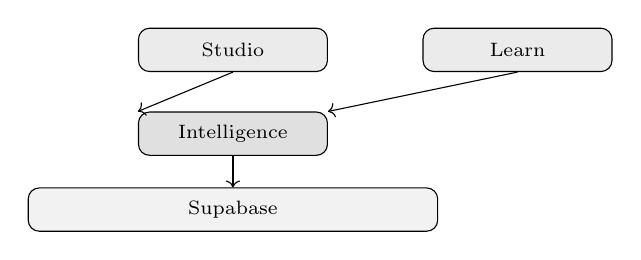
\begin{tikzpicture}[node distance=0.35cm and 0.5cm, every node/.style={font=\scriptsize},
  layer/.style={rectangle, draw, rounded corners, minimum height=0.55cm, inner sep=3pt}]
  \node[layer, fill=black!8, minimum width=2.4cm] (studio) {Studio};
  \node[layer, fill=black!8, minimum width=2.4cm, right=1.2cm of studio] (learn) {Learn};
  \node[layer, fill=black!12, minimum width=2.4cm, below=0.5cm of studio] (intel) {Intelligence};
  \node[layer, fill=black!5, minimum width=5.2cm, below=0.4cm of intel] (data) {Supabase};
  \draw[->] (studio.south) -- (intel.north west);
  \draw[->] (learn.south) -- (intel.north east);
  \draw[->] (intel.south) -- (data.north);
\end{tikzpicture}%
}
\caption{Reference platform: Studio, Learn, Intelligence, shared data.}
\label{fig:arch}
\end{figure}

\subsection{Digital Learner Twin and Learner Model}
\label{sec:twin}

A persistent \textbf{Digital Learner Twin} is stored in \texttt{learner\_profiles}. It includes: modality affinity scores (per format), learning pace and difficulty comfort, behavioral signals (session duration, completion rate, streak), and an \texttt{ai\_tutor\_context} JSON field holding known concepts, struggles, learning-style notes, goals, and interaction summaries. This context is updated asynchronously from tutor interactions and quiz outcomes (e.g., struggle detection). The design aligns with open learner model principles \cite{bull2016} and supports personalization across courses and sessions.

\subsection{AI Tutor with Longitudinal Memory}
\label{sec:tutor}

The AI tutor (named Sudar in the reference implementation) is reactive (RAG over course content, answers questions) and proactive (nudges when struggle or long pause is inferred). Every exchange is logged in \texttt{ai\_interactions}. The tutor's system prompt includes the learner's memory summary from \texttt{ai\_tutor\_context}, so responses can reference prior struggles, match explanation style, and connect to prior learning. Most ``AI in LMS'' implementations are stateless; ours is not.

\subsection{Modality-Agnostic Delivery}
\label{sec:modality}

Content is authored once (courses and modules with structured content). The delivery layer can present the same material as text, video, audio, mindmap, flashcards, a feed-style view, or a game. A modality dispatcher (in Intelligence) can recommend the next modality from the learner's profile and behavior. This supports dual coding and learner agency \cite{mayer2009,clark2016}. Text and flashcards are fully implemented; video, audio, mindmap, feed, and game are in progress or planned.

\subsection{Adaptive Sequencing and Next-Best Action}
\label{sec:adaptive}

Learning paths support mandatory and optional courses and unlock rules (complete previous before next). For optional courses, the order can be adapted by the engine from the learner profile and gaps. A next-best-action algorithm suggests the next course or module and explains why, surfacing required and due-soon items. Formative assessment (in-module quizzes with immediate feedback) and struggle detection feed the learner model \cite{black1998,roediger2006}.

\subsection{Plugin Architecture for Existing LMSs (ALP)}
\label{sec:alp}

The \textbf{Adaptive Learning Layer (ALP)} is the design by which the same capabilities can be offered to existing LMSs without replacing them. Conceptually, ALP comprises: (1) a \textbf{learner model API} that maintains or syncs a longitudinal profile from LMS events; (2) a \textbf{tutor service} that uses that profile and course content for memory-aware Q\&A and nudges; (3) a \textbf{modality layer} that can deliver or recommend alternative formats for content already in the LMS. Integration points: the LMS sends learning events and (optionally) content references to ALP; ALP returns next-best-action, tutor responses, and modality recommendations. To our knowledge, no widely adopted technology today adds longitudinal learner model and memory-aware tutoring to incumbent LMSs in a pluggable way; ALP is designed to fill that gap. The reference platform serves as the proof-of-concept and open-source reference for ALP.\footnote{Reference implementation: Sudar (repository: \url{https://github.com/lorddannykay/ByteOS}).} Figure~\ref{fig:alp} illustrates the ALP concept: existing LMSs keep hosting content and enrollments; ALP adds learner model, tutor, and modality layer via APIs and events.
\begin{figure}[t]
\centering
\resizebox{0.85\columnwidth}{!}{%
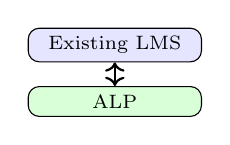
\begin{tikzpicture}[node distance=0.3cm, every node/.style={font=\scriptsize},
  layer/.style={rectangle, draw, rounded corners, inner sep=3pt}]
  \node[layer, fill=blue!10, minimum width=2.2cm] (lms) {Existing LMS};
  \node[layer, fill=green!15, minimum width=2.2cm, below=0.3cm of lms] (alp) {ALP};
  \draw[<->, thick] (lms.south) -- (alp.north);
\end{tikzpicture}%
}
\caption{ALP as a layer on top of an existing LMS.}
\label{fig:alp}
\end{figure}

\section{Implementation and Reproducibility}
\label{sec:impl}

The reference platform is implemented with Next.js~14 (Studio, Learn), Python~3.11+ FastAPI (Intelligence), and Supabase (PostgreSQL, auth, storage). AI providers include Together AI (primary), OpenAI, and Anthropic. The schema and event model are documented in the repository (ECOSYSTEM.md, RESEARCH\_FOUNDATION.md). Key tables: \texttt{learner\_profiles}, \texttt{learning\_events}, \texttt{ai\_interactions}, \texttt{enrollments}, \texttt{certifications}. The project is open source (MIT). We provide a citation in the repository and in Section~\ref{sec:eval} for reproducibility and derivative work.

\section{Evidence and Evaluation Strategy}
\label{sec:eval}

\paragraph{Research foundation.}
The design is evidence-informed. RESEARCH\_FOUNDATION.md in the repository maps each capability to learning-science references (adaptive instruction, dual coding, self-regulated learning, formative assessment, ITS, learner modeling).

\paragraph{Proof of concept.}
The reference platform currently implements: shared auth and schema; course and path CRUD and publish; learner dashboard with streak, time, and Sudar recommends; course viewer with markdown, quizzes, and AI tutor with longitudinal memory (My Memory page, text selection to tutor); next-best-action and adaptive path ordering; learning paths with unlock rules and certifications with shareable links; compliance view (overdue, at-risk, on-track); analytics (completions, quiz scores, struggle topics, time per section). Flashcards modality and document-to-course generation are implemented; SCORM import is in progress. Additional modalities (video, audio, mindmap, feed, game) are planned.

\begin{center}
\fbox{\parbox{0.9\columnwidth}{
\textbf{Call for collaboration.} We invite institutions and organizations to collaborate on pilots and plugin integrations with the reference platform or with ALP components for existing LMSs. We are open to reporting anonymized early adopters and aggregate outcomes in a follow-up or extended version of this work. Contact and collaboration details are available in the repository: \url{https://github.com/lorddannykay/ByteOS}.
}}
\end{center}

\paragraph{Pilot in progress.}
A pilot evaluation is being conducted in partnership with an organizational partner to assess adoption and learning outcomes. The pilot is independent of the design and ownership of the system; the system and research remain the authors' project. Results will be reported in a subsequent paper when available.

\section{Discussion}
\label{sec:discussion}

\paragraph{Limitations.}
Not all modalities are yet fully implemented; plugin integrations with specific LMSs are not yet in production. Efficacy data from the reference platform and from ALP deployments will strengthen the claims in future work.

\paragraph{Future work.}
We plan to extend modalities, add LMS-specific connectors for ALP, run controlled efficacy studies, and support more organizational features (e.g., SSO, HRIS hooks) where needed.

\paragraph{Goal.}
Our goal is to make learning accessible and adaptive at scale---both through the reference platform and by enabling existing LMSs to become adaptive, memory-aware learning experience platforms via ALP.

\section{Conclusion}
\label{sec:conclusion}

We presented an AI-native learning system with two contributions: a reference platform that combines authoring, delivery, and intelligence with a Digital Learner Twin, adaptive sequencing, multimodal delivery, and an AI tutor with longitudinal memory; and the Adaptive Learning Layer (ALP), an architecture for deploying these capabilities as a layer on top of existing LMSs. The reference implementation is open source and evidence-informed. We invite collaboration from institutions and organizations so that learning can become accessible and adaptive for everyone.

\section*{Acknowledgments}
The system and research are the authors' project. The reference implementation is available at \url{https://github.com/lorddannykay/ByteOS} with documentation (ECOSYSTEM.md, RESEARCH\_FOUNDATION.md, docs/sudar-memory.md). The platform is named Sudar.

\appendix
\section{Schema summary}
Key tables for reproducibility: \texttt{learner\_profiles} (Digital Learner Twin: \texttt{ai\_tutor\_context}, \texttt{next\_best\_action}, modality scores, behavioral signals); \texttt{learning\_events} (event\_type, payload, modality, duration); \texttt{ai\_interactions} (user\_message, ai\_response, context\_used); \texttt{enrollments} (path/course, progress, due\_date); \texttt{certifications}. Full schema: ECOSYSTEM.md in the repository.

\bibliographystyle{plain}
\bibliography{references}
\end{document}
